% questions.tex —— 1978 年·全国卷 · 题目内容片段（无答案）
% 由 tools/generate_projects.py 依来源总账自 1978/1978_数学真题_全国_试题.md 生成，勿手改（改源 MD 后重跑）


\begin{gktip}
\textbf{来源说明}：本卷为文理合卷，单页（原卷页码第 12 页），全卷共 7 题。固定原卷文件名标注“5、6 选做一题，文科不做第 7 题”，据此本卷第 5 题为三角与解三角形、第 6 题为三角恒等式证明，二者由考生\textbf{选做一题}；第 7 题（二次函数与抛物线）\textbf{文科考生不作}。本文按原卷题号 1—7 逐题转录，未作重编号，选做/免做规定一并保留。

\textbf{题面说明}：本卷题面不含答案（答案由本库独立推导）。第 3 题依原卷配图重绘为 TikZ 矢量图。

\textbf{源注}：第 2 题原卷印作“分别指出方程所代表图形的\textbf{内形}”，其中“内形”当为“形状”之排印误（\texttt{pdftotext} 文本层与页面图像均作“内形”），本文保留原字面，未径改。
\end{gktip}

\begin{question}
\gkti{1}（1） 分解因式：$x^2-4xy+4y^2-4z^2$。

（2） 已知正方形的边长为 $a$，求侧面积等于这个正方形的面积、高等于这个正方形边长的直圆柱体的体积。

（3） 求函数 $y=\sqrt{\lg(2+x)}$ 的定义域。

（4） 不查表求 $\cos 80^\circ\cos 35^\circ+\cos 10^\circ\cos 55^\circ$ 的值。

\Needspace{5\baselineskip}
（5） 化简
\nopagebreak[4]
\[
\left(\frac14\right)^{-\frac12}\cdot\frac{\left(\sqrt{4ab^{-1}}\right)^3}{(0.1)^{-2}\left(a^3b^{-4}\right)^{\frac12}}.
\]

\end{question}
\begin{question}
\gkti{2}已知方程 $kx^2+y^2=4$，其中 $k$ 为实数。对于不同范围的 $k$ 值，分别指出方程所代表图形的内形，并画出显示其数量特征的草图。

\Needspace{0.4\textheight}
\end{question}
\begin{question}
\gkti{3}如图，$AB$ 是半圆的直径，$C$ 是半圆上一点，直线 $MN$ 切半圆于 $C$ 点，$AM\perp MN$ 于 $M$ 点，$BN\perp MN$ 于 $N$ 点，$CD\perp AB$ 于 $D$ 点。求证：

（1） $CD=CM=CN$；

（2） $CD^2=AM\cdot BN$。
\nopagebreak[4]
\begin{center}% 1978 年全国卷第 3 题：半圆（直径 AB），C 在弧上，MN 切半圆于 C，AM⊥MN 于 M、BN⊥MN 于 N、CD⊥AB 于 D（按源卷布局）
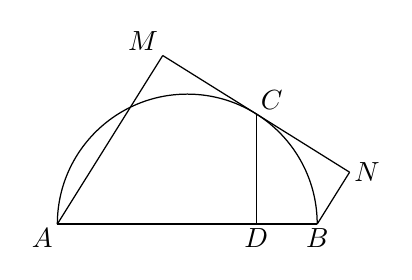
\begin{tikzpicture}[scale=1.65, line width=0.45pt,
  every node/.style={inner sep=1.5pt}]
  \coordinate (A) at (-1,0);
  \coordinate (B) at (1,0);
  \coordinate (C) at (0.53,0.848);
  \coordinate (D) at (0.53,0);
  \coordinate (M) at (-0.189,1.297);
  \coordinate (N) at (1.249,0.399);
  \draw (A) arc (180:0:1);
  \draw (A) -- (B);
  \draw (M) -- (N);
  \draw (A) -- (M);
  \draw (B) -- (N);
  \draw (C) -- (D);
  \node[anchor=south east] at (M) {$M$};
  \node[anchor=south west] at (C) {$C$};
  \node[anchor=west] at (N) {$N$};
  \node[anchor=north east] at (A) {$A$};
  \node[anchor=north] at (D) {$D$};
  \node[anchor=north] at (B) {$B$};
\end{tikzpicture}
\end{center}
\nopagebreak[4]
\end{question}
\begin{question}
\gkti{4}已知 $\log_{18}9=a$，$18^b=5$，求 $\log_{36}45$。

\end{question}
\begin{question}
\gkti{5}已知 $\triangle ABC$ 的三个内角的大小成等差数列，$\tan A\tan C=2+\sqrt3$，求角 $A$、$B$、$C$ 的大小。又已知顶点 $C$ 的对边 $c$ 上的高等于 $4\sqrt3$，求三角形各边 $a$、$b$、$c$ 的长。（提示：必要时可验证 $(1+\sqrt3)^2=4+2\sqrt3$）

\end{question}
\begin{question}
\gkti{6}已知 $\alpha$、$\beta$ 为锐角，$3\sin^2\alpha+2\sin^2\beta=1$，$3\sin 2\alpha-2\sin 2\beta=0$。求证：
\nopagebreak[4]
\[
\alpha+2\beta=\frac{\pi}{2}.
\]

\end{question}
\begin{question}
\gkti{7}已知函数 $y=x^2+(2m+1)x+m^2-1$（$m$ 为实数）。

（1） $m$ 是什么数值时，$y$ 的极值是 $0$？

（2） 求证：不论 $m$ 是什么数值，函数图象（即抛物线）的顶点都在同一条直线 $L_1$ 上，画出 $m=-1$、$0$、$1$ 时抛物线的草图，来检验这个结论；

（3） 平行于 $L_1$ 的直线中，哪些与抛物线相交，哪些不相交？求证：任一条平行于 $L_1$ 而与抛物线相交的直线，被各抛物线截出的线段都相等。

\end{question}